\documentclass[a4paper,10pt]{article}

\usepackage[margin=2cm]{geometry}
\usepackage{graphicx}
\usepackage{amsmath}
\usepackage{array}
\usepackage{hyperref}
\usepackage[all]{hypcap}
\usepackage{listings}
\lstdefinestyle{TerminalStyle}{
  language=bash,
  basicstyle=\small\sffamily,
  numbers=left,
  numberstyle=\tiny,
  numbersep=3pt,
  frame=tb,
  columns=fullflexible,
  linewidth=0.9\linewidth,
  xleftmargin=0.1\linewidth
}
\lstdefinestyle{HtmlStyle}{
  language=html,
  basicstyle=\small\sffamily,
  numbers=left,
  numberstyle=\tiny,
  numbersep=3pt,
  frame=tb,
  columns=fullflexible,
  linewidth=0.9\linewidth,
  xleftmargin=0.1\linewidth
}
\lstdefinestyle{OutputStyle}{
  language=html,
  basicstyle=\small\sffamily,
  frame=tb,
  columns=fullflexible,
  linewidth=0.9\linewidth,
  xleftmargin=0.1\linewidth
}


\usepackage[margin=2cm]{geometry}
\usepackage{graphicx}
\usepackage{amsmath}
\usepackage{array}
\usepackage{hyperref}
\usepackage[all]{hypcap}
\usepackage{listings}
\lstdefinestyle{TerminalStyle}{
  language=bash,
  basicstyle=\small\sffamily,
  numbers=left,
  numberstyle=\tiny,
  numbersep=3pt,
  frame=tb,
  columns=fullflexible,
  linewidth=0.9\linewidth,
  xleftmargin=0.1\linewidth
}
\lstdefinestyle{HtmlStyle}{
  language=html,
  basicstyle=\small\sffamily,
  numbers=left,
  numberstyle=\tiny,
  numbersep=3pt,
  frame=tb,
  columns=fullflexible,
  linewidth=0.9\linewidth,
  xleftmargin=0.1\linewidth
}
\lstdefinestyle{OutputStyle}{
  language=html,
  basicstyle=\small\sffamily,
  frame=tb,
  columns=fullflexible,
  linewidth=0.9\linewidth,
  xleftmargin=0.1\linewidth
}

\setlength{\parindent}{0pt}
\setlength{\parskip}{1ex plus 0.5ex minus 0.2ex}
\title{
\includegraphics[width=13cm]{CodeXBanner2rounded.jpg} \\
       \vspace{0.2cm}
       \begin{large}
       
\includegraphics[width=13cm]{UserManual.jpg} \\
       \end{large}
       }
       
       \vspace{50cm}

\date{} 
\author{	Bondjobo, Jocelyn 		13232852 		\\
		Malangu, Daniel		13315120		\\
		Kirker, Tim			11152402		\\
		Hammond, Eunice	NK	13222563		\\
		Burgers, Heinrich		15059538		\\
}

\begin{document}
\maketitle
\thispagestyle{empty}
\clearpage

\newpage
\pagenumbering{roman}
\thispagestyle{empty}
\tableofcontents
\clearpage

\newpage
\pagenumbering{arabic}


\section{Introduction}
Reroute Systems is a software company with different in-house developed applications. The Purchase Management System 
application specifically, is the main application and is mainly active in the pharmaceutical space.\\
This document contains guidelines on how the application works, and how one can maximise the application and all it entails for best use.\\

\section{General Information}
\subsection{About}
This application is the Reroute Purchasing Management System affiliated with the Reroute Systems company.\

For best use, it is advised that users have background knowledge in the pharmaceutical space.\\

\subsection{System Overview}
The system is a search engine called \textbf{Smart Search Pharmaceutical} which is enriched with functionality. Our system allows the user to customize how the search algorithm relates words to each other. This allows the user to search for a term as well as terms related to it, with different spellings and different variations of the term. Our system allows the user to retrieve specific records from very large amounts of data in a very small amount of time. 

	\subsubsection{Stakeholders}
	The stakeholders of the system include the following:
	\begin{itemize}
	\item \textbf{The Client} is Diederik Mostert, Software Director of ReRoute Systems who proposed the project as a result of a challenge faced in the company, which is to search a product on master file with different combination used by each wholesaler.
	\item \textbf{Users in Pharmaceutical space} They will use the system to retrieve information of the product they need.
	\end{itemize}
\subsection{System Configuration}
	{\centering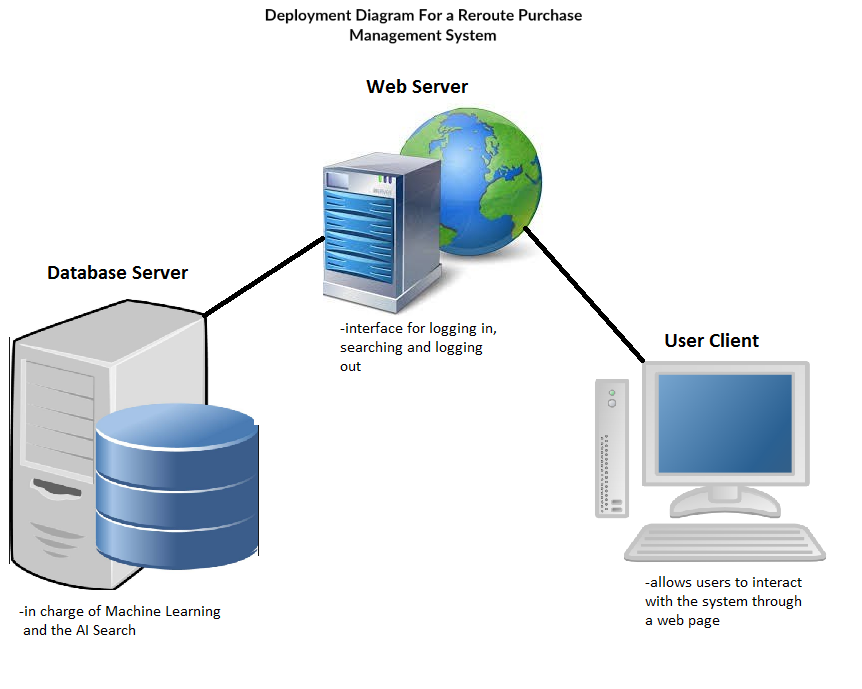
\includegraphics[width=15cm, scale=0.5]{User Manual Deployment diagram.png}} \\

\subsection{Note to the User}
This system allows the user to search for a word and related terms. It also allows the user to link words to each other. This allow the user to customize their experience to their needs. For example, one can link words like "Panado" to "Grandpas", or "Panado" to "headache", so that if one were to search "headache", one would also receive the results for "Panados" and "Grandpas". This is made possible through the use of a dictionary. To get the ultimate experience, it is advised that as a user you make use of this dictionary by linking terms are deemed related that they wish to have linked.

\subsection{Installation}
To be defined.

\section{Getting started}
	The application design looks as follows: \\
	\subsection{Main Screen}
	When the application is launched it requires your log-in credentials.\\
	{\centering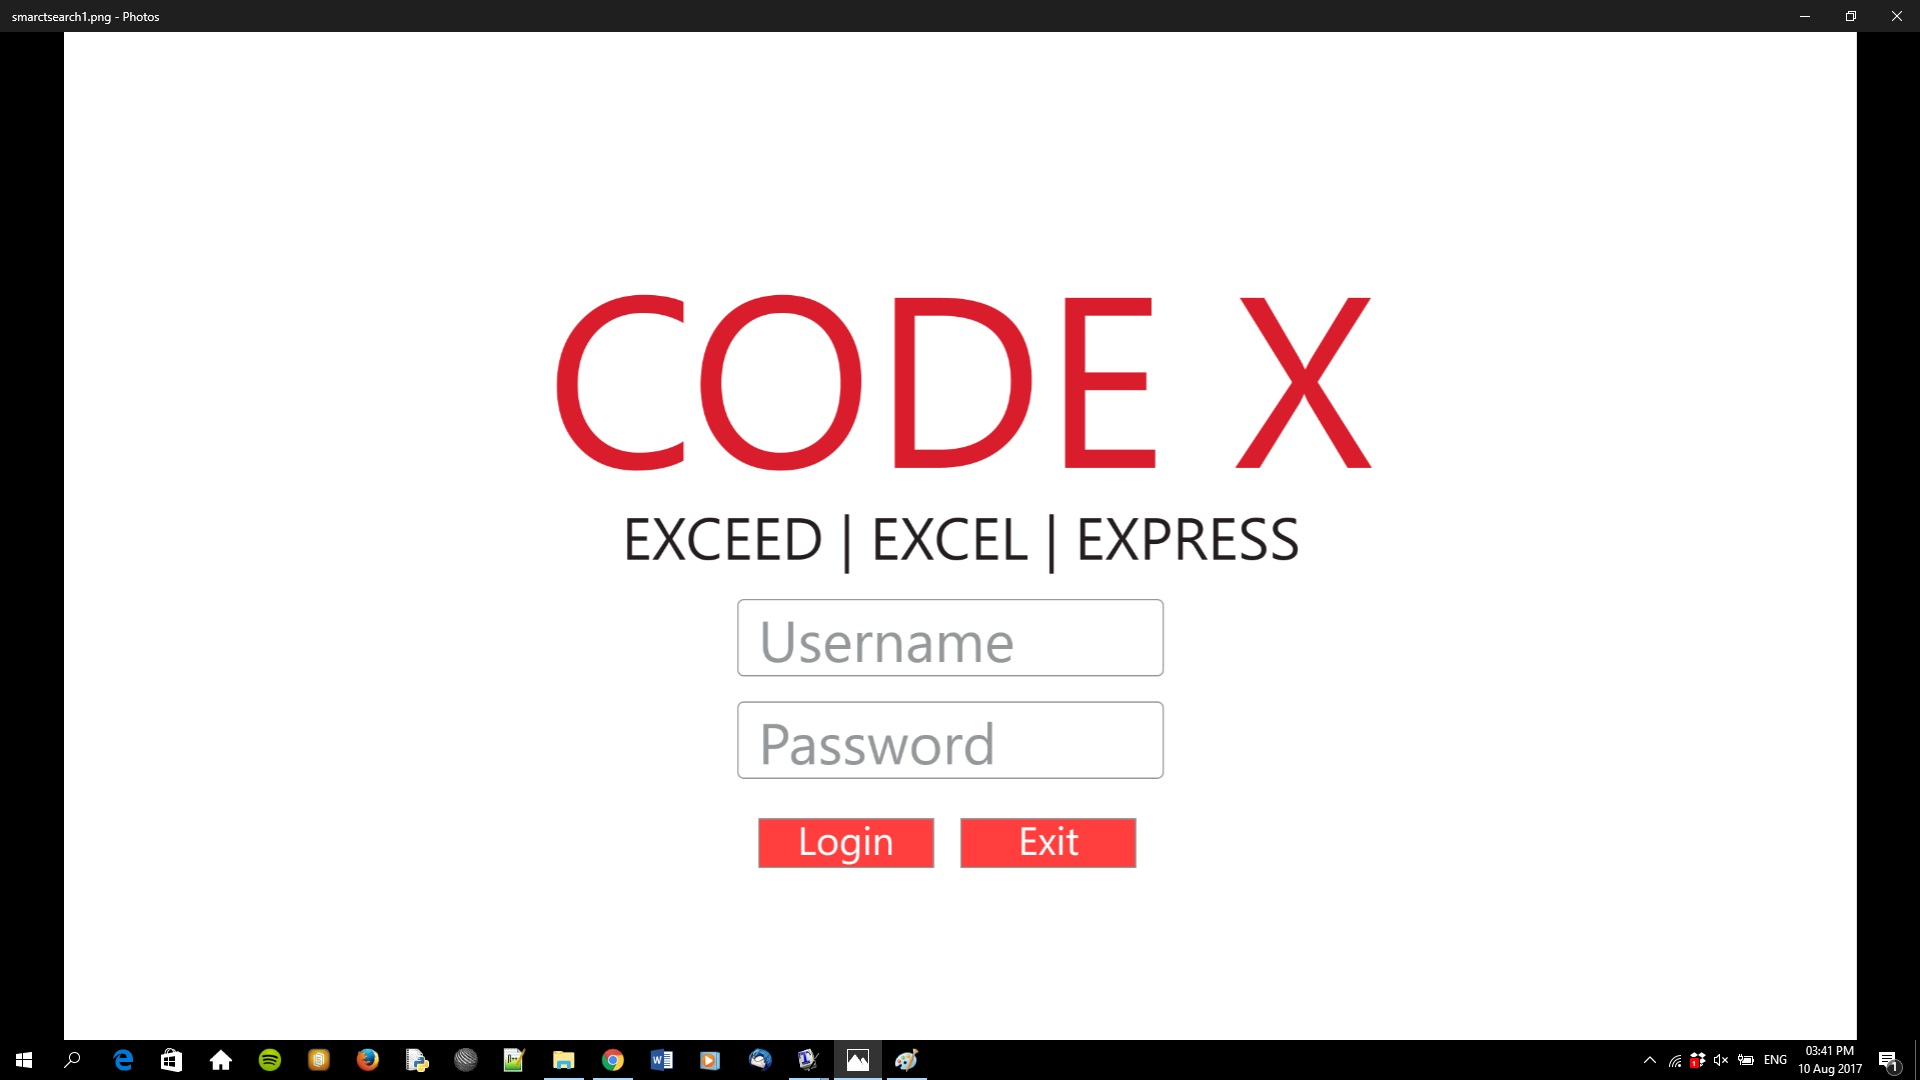
\includegraphics[width=15cm, scale=0.5]{smarctsearch1.jpg}}
	\subsection{Pharmaceutical Search Menu}
	The search screen where the user enters the product information to search on. \\
	{\centering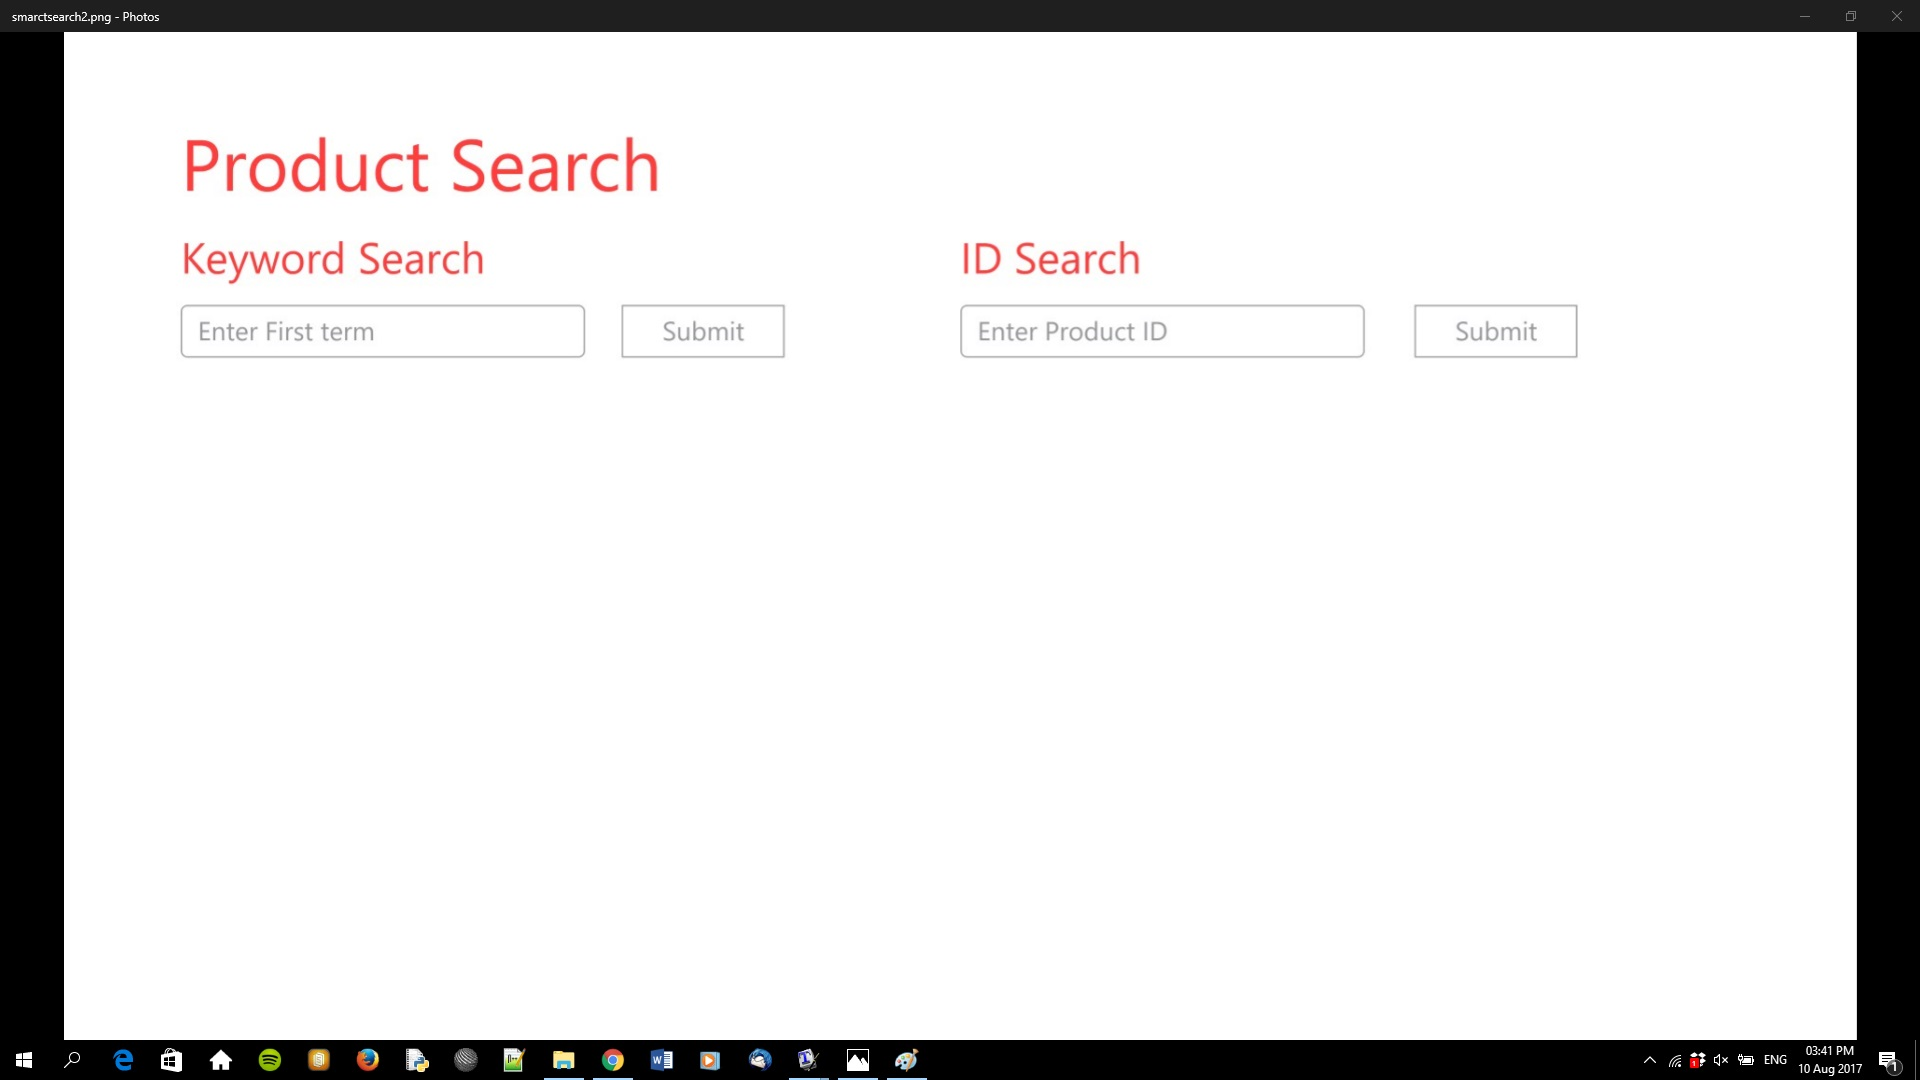
\includegraphics[width=15cm, scale=0.5]{smarctsearch2.jpg}} \\ \\
	{\centering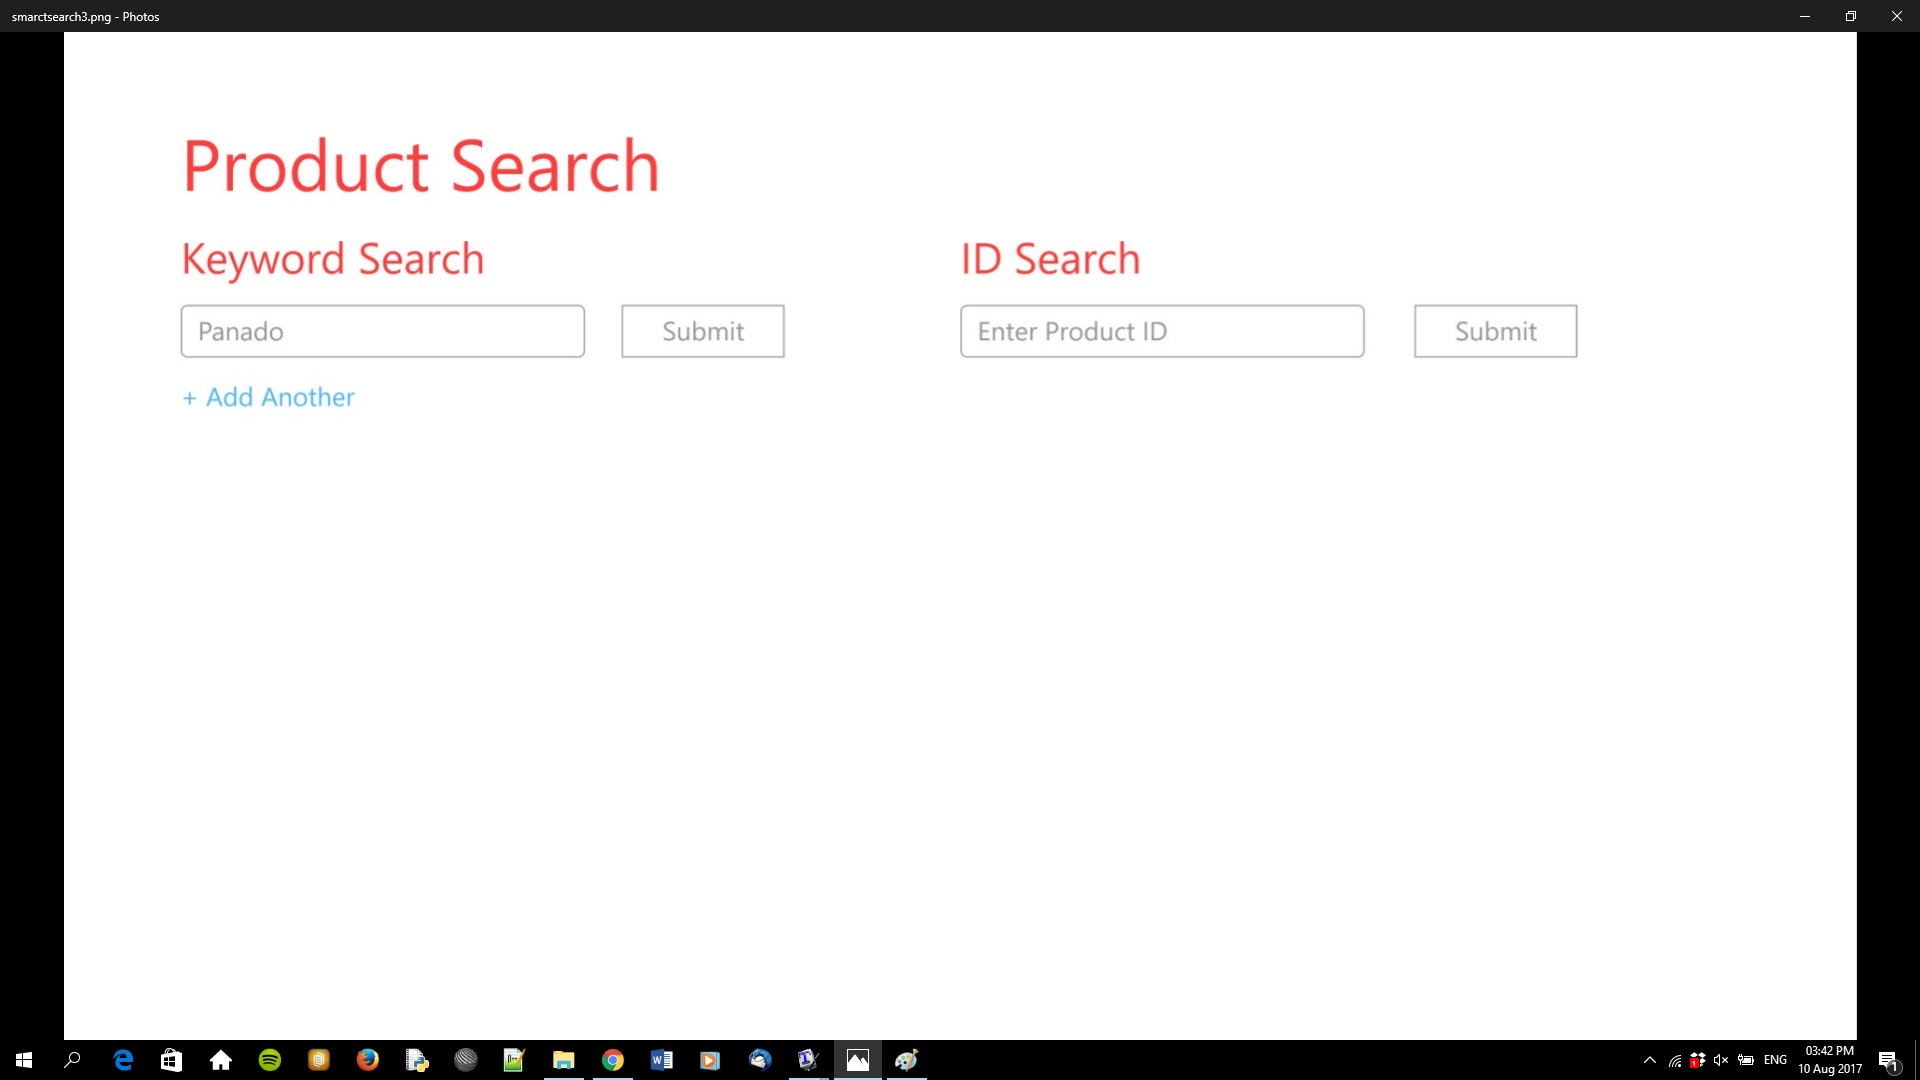
\includegraphics[width=15cm, scale=0.5]{smarctsearch3.jpg}} \\ \\
	{\centering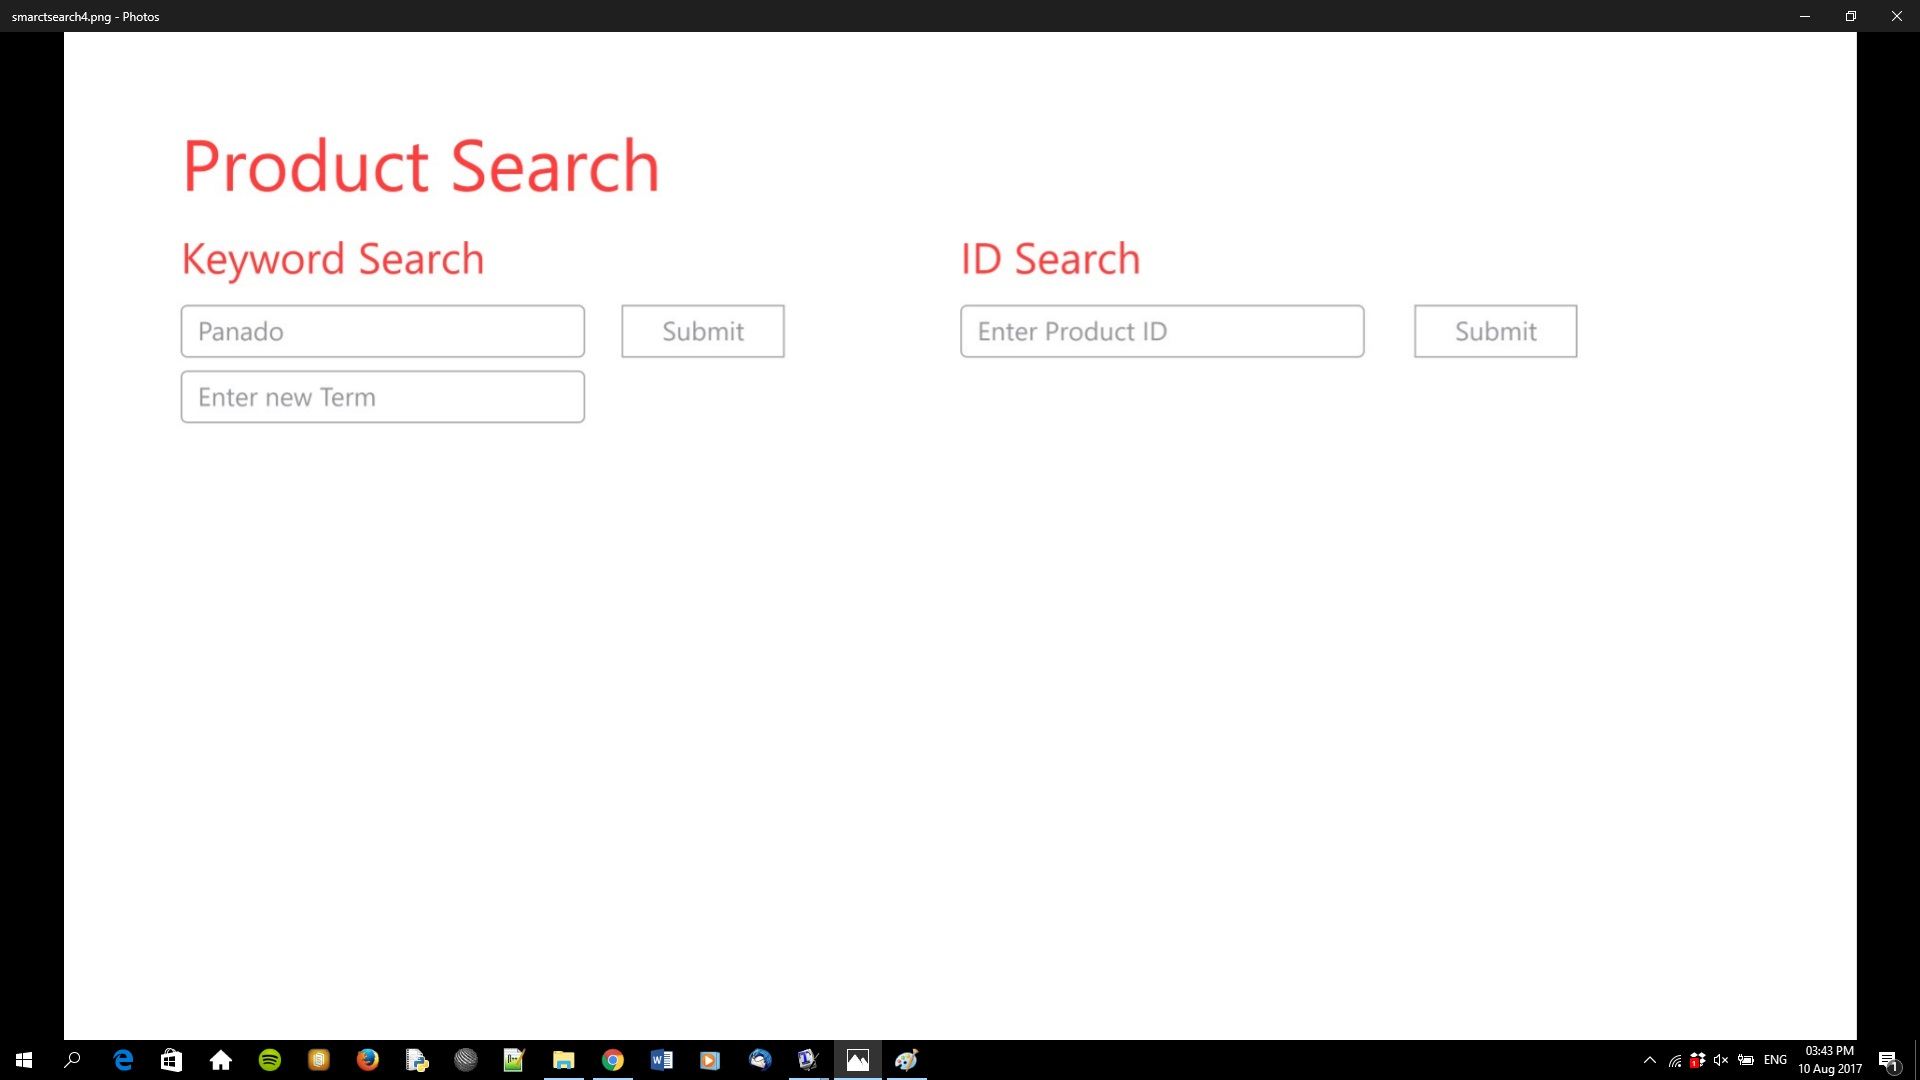
\includegraphics[width=15cm, scale=0.5]{smarctsearch4.jpg}} \\ \\
	{\centering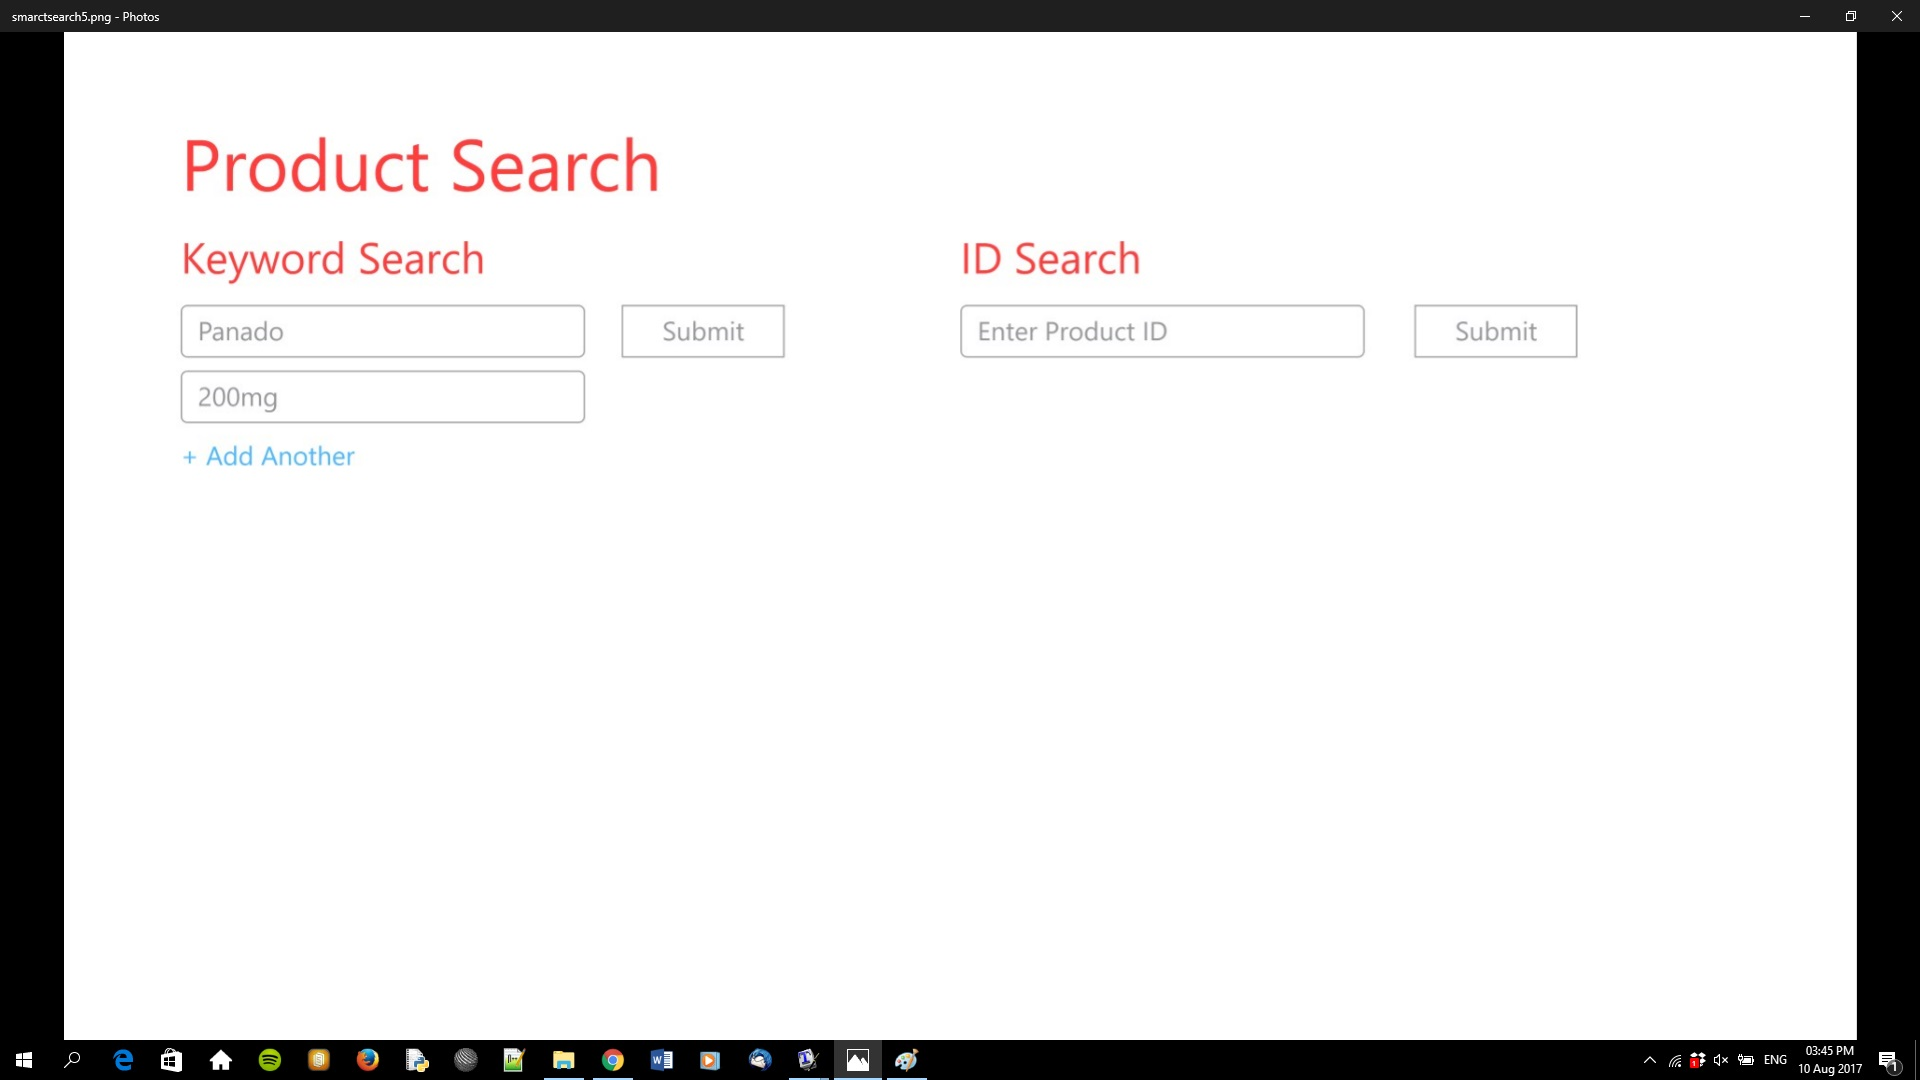
\includegraphics[width=15cm, scale=0.5]{smarctsearch5.jpg}} \\
	\subsection{Search Result}
	The result of a search would yield a result below: \\
	{\centering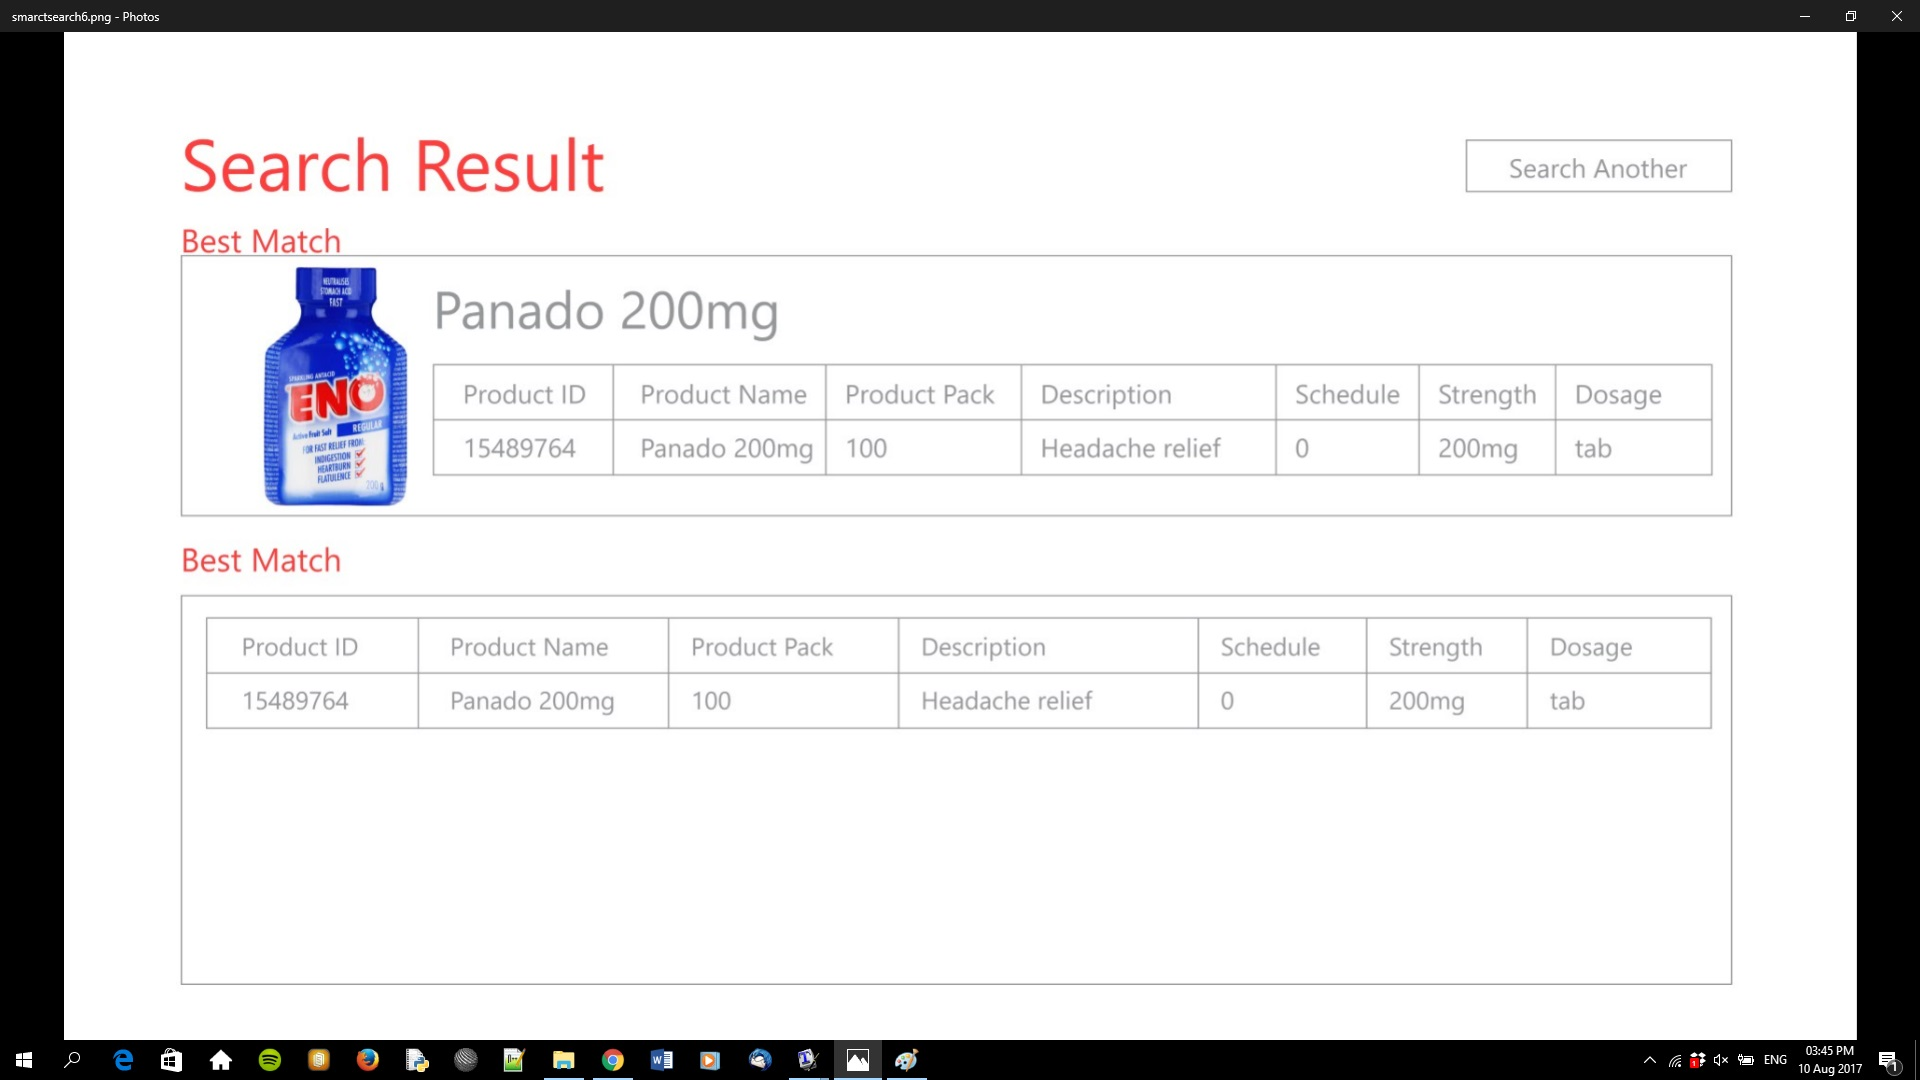
\includegraphics[width=15cm, scale=0.5]{smarctsearch6.jpg}} \\
	
\section{Using the System}
	After registering yourself as a user, you can use the following actions to use the system:
	\begin{enumerate}
	\item \textbf{Logging In:}
		After running the program, you will be presented with a log-in screen.  In this screen, you will need to provide your $username$ and $password$ to gain access to your account.
	\item \textbf{Menu:}
		After logging in, you will be presented with a screen containing the different options a user can take. These options are \textbf{(1) Search Product, (2) Edit Dictionary, (3) Dictionary,} and \textbf{ (4) Delete Product.}

	\item \textbf{Search:}
		On this screen, you will be presented with an option to search a product by \textbf{name} or by \textbf{ID}. If you would like to search by name, type the name or a term related to it, and press the search button. If you would like to search by ID, you need to type the exact ID and then press search.  After pressing search, you will be presented with either possible matches to your search or the exact match to the ID.  From here, you can select products you are interested in to order.
	\item \textbf{Edit Dictionary:}
		At the "Edit Dictionary" screen, you can see the words already added to the dictionary. Here, you can delete words that you would prefer not to be linked at all.
	\item \textbf{View Dictionary:}
		On the "Dictionary" screen, you can add words to the dictionary that you would like to be linked. For example, you can link the word "TABS" to "TABLETS" by inserting the word "TABS" in the left text-box, and the word "TABLETS" in the right text-box. These words will now be linked and both will be included in the result space when searched for. 
	\item \textbf{Delete Record:}
		At this option, the user can delete data from the tables. 
	\item \textbf{Log-out:}
		After placing an order and have no more to do, remember to log-out. To do so, simply press the "Log-out" button.\\
	\end{enumerate}
	
\section{Troubleshooting}
	Please report any errors found with this system to allow development teams to correct it. If you wish to do so yourself, here are some useful things to look at:

	\begin{enumerate}
		\item \textbf{General Issues:}\\\
			Most issues can be fixed by simply restarting the program or your computer. 
		\item \textbf{Error communicating to the database:}\\\
			The database system in use, ZIZO, makes use of SOAP and REST calls to communicate with the rest of the system. Ensure that the system has an internet connection. If you do have an internet connection, ensure that the system is communicating with the database system. 
		\item \textbf{System crashes:}\\\
			Please report any areas or actions that cause(d) the system to crash to the developers.
		\item \textbf{Faulty data:}\\\
			Reading data into the database is an automated process and faulty data often gets through. Please report such cases to Catura Reroute Systems.
	\end{enumerate}
	

\end{document}
